%%%This is a science homework template. Modify the preamble to suit your needs. 

\makeatother
\input{../templates/packages.tex}
\input{../templates/theorems.tex}
\input{../templates/macros.tex}
%
%Redefining sections as problems
%
\makeatletter
\newenvironment{problem}{\@startsection
       {section}
       {1}
       {-.2em}
       {-3.5ex plus -1ex minus -.2ex}
       {2.3ex plus .2ex}
       {\pagebreak[3]%forces pagebreak when space is small; use \eject for better results
       \large\bf\noindent{Problem }
       }
       }
       {%\vspace{1ex}\begin{center} \rule{0.3\linewidth}{.3pt}\end{center}}
       }
\makeatother

\renewcommand{\div}{\operatorname{div}}
%
%Fancy-header package to modify header/page numbering 
%
\usepackage{fancyhdr}
\pagestyle{fancy}
%\addtolength{\headwidth}{\marginparsep} %these change header-rule width
%\addtolength{\headwidth}{\marginparwidth}
\lhead{Problem \thesection}
\chead{} 
\rhead{\thepage} 
\lfoot{\small\scshape 18.404 Theory of Computation} 
\cfoot{} 
\rfoot{\small PS \# 1} % !! Remember to change the problem set number
\renewcommand{\headrulewidth}{.3pt} 
\renewcommand{\footrulewidth}{.3pt}
\setlength\voffset{-0.25in}
\setlength\textheight{648pt}



%%%%%%%%%%%%%%%%%%%%%%%%%%%
%
%Contents of problem set
%    
\begin{document}
\title{18.404 Theory of Computation PSet\#1}% !! Remember to change the problem set number
\author{Holden Lee}
\date{9/15/12}% !! Remember to change the date
\maketitle
%\thispagestyle{empty}
\begin{problem}{\it (1.32, Parallel addition)}
I first show that $B^{\cal R}$ is regular. I claim that the following DFA recognizes $B^{\cal R}$:

\tikzstyle{state}=[circle,draw,inner sep=1pt,minimum size=6mm]
\tikzstyle{accept}=[circle,draw,inner sep=4pt,minimum size=7.5mm]
\begin{center}
\begin{tikzpicture}[->,>=stealth',shorten >=1pt,auto,node distance=1cm,semithick]
\node (start) [state] {start};
\node (start) [accept] {start};
\node (regroup) at (4,0) [state] {regroup};
\node (dead) at (2,-2) [state] {dead};
\node (0) at (-2,0) {};
\path (0) edge node {} (start);
\path (start) edge [loop above] node {$\scriptsize\colthree000,\colthree011,\colthree 101$} (start); 
\path (start) edge [bend right] node {$\scriptsize\colthree110$}(regroup) ;
\path (start) edge [swap] node {$\scriptsize\colthree001,\colthree111,\colthree 110,\colthree 010$}(dead) ;
\path (dead) edge [loop below] node {all}(dead) ;
\path (regroup) edge node{$\scriptsize\colthree 000,\colthree011,\colthree101,\colthree110$} (dead) ;
\path (regroup) edge [loop right] node {$\scriptsize\colthree010,\colthree100,\colthree111$}(regroup) ;
\path (regroup) edge [bend right,swap] node {$\scriptsize\colthree001$} (start);
\end{tikzpicture}
\end{center}
The idea is that the machine will be at the start state when ``everything adds up right so far," at the regroup state when it's carrying a 1, and dead when there is no hope of the first two binary numbers adding up to the third.

More precisely, for a word $w\in \Si_3^*$, let $w_1,w_2,w_3$ be the binary numbers obtained from reading the first, second, and third rows respectively. For integers $m\ne 0, a$, let $a\pmod m$ be the unique number in $[0,m)$ with same residue as $a$. 
\begin{clm}
\begin{enumerate}
\item
if the machine is at ``start" at the $n$th step, then
\[
w_1\md{2^n}+w_2\md{2^n}=w_3\md{2^n}
\]
\item
if the machine is at ``regroup" at the $n$th step, then
\[
w_1\md{2^n}+w_2\md{2^n}=w_3\md{2^n}+2^n
\]
\item
if the machine is at ``dead" at the $n$th step, then
\[
w_1+w_2\nequiv w_3\pmod{2^n}.
\]
\end{enumerate}
\end{clm}
\begin{proof}
The proof is by induction. At step $n=0$, the machine is in the start state and $2^n=1$, so the statement clearly holds.

Suppose the claim true for $n$, and we're reading the next symbol $a_{n+1}=\colthree{a_{n+1,1}}{a_{n+1,2}}{a_{n+1,3}}$ Consider 3 cases.
\begin{enumerate}
\item
We are at the start state.
\begin{itemize}
\item
$a_{n+1}=\colthree000,\colthree011,\colthree101$. Note in these cases, $a_{n+1,1}+a_{n+1,2}=a_{n+1,3}$, so
\bal
w_1\md{2^{n+1}}+w_2\md{2^{n+1}}&=w_1\md{2^n} +w_2\md{2^n}+2^n(a_{n+1,1}+a_{n+1,2})\\
&=w_3\md{2^n}+2^na_{n+1,3}\\
&=w_3\md{2^{n+1}}
\end{align*}
which is consistent with the fact that we follow the loop back to ``start."
\item
$a_{n+1}=\colthree110$. We have
\bal
w_1\md{2^{n+1}}+w_2\md{2^{n+1}}&=w_1\md{2^n} +w_2\md{2^n}+2^n(1+1)\\
&=w_3\md{2^{n}}+2^{n+1}\\
&=w_3\md{2^{n+1}}+2^{n+1}
\end{align*}
which is consistent with the fact that we are now at ``regroup."
\item
$a_{n+1}=\colthree001,\cth001,\cth111,\cth010$. In these cases, $a_{n+1,1}+a_{n+1,2}\nequiv a_{n+1,3}\pmod 2$, so
\bal
w_1\md{2^{n+1}}+w_2\md{2^{n+1}}&=w_1\md{2^n} +w_2\md{2^n}+2^n(a_{n+1,1}+a_{n+1,2})\\
&\nequiv w_3\md{2^n}+2^na_{n+1,3}\pmod{2^{n+1}}\\
&\equiv w_3\md{2^{n+1}}\pmod{2^{n+1}},
\end{align*}
which is consistent with the fact we are now at ``dead."
\end{itemize}
\item We are at the regroup state.
\begin{itemize}
\item
$a_{n+1}=\colthree010,\colthree100,\colthree111$. Note in these cases, $a_{n+1,1}+a_{n+1,2}=a_{n+1,3}+1$, so
\bal
w_1\md{2^{n+1}}+w_2\md{2^{n+1}}&=w_1\md{2^n} +w_2\md{2^n}+2^n+2^n(a_{n+1,1}+a_{n+1,2})\\
&=w_3\md{2^n}+2^n(a_{n+1,3}+1)+2^{n}\\
&=w_3\md{2^{n+1}}+2^{n+1}
\end{align*}
which is consistent with the fact that we follow the loop back to  ``regroup."
\item
$a_{n+1}=\colthree001$. We have
\bal
w_1\md{2^{n+1}}+w_2\md{2^{n+1}}&=w_1\md{2^n} +w_2\md{2^n}+2^n\\
&=w_3\md{2^{n+1}}
\end{align*}
which is consistent with the fact that we are now at ``start."
\item
$a_{n+1}=\colthree 000,\colthree011,\colthree101,\colthree110$. In these cases, $a_{n+1,1}+a_{n+1,2}\equiv a_{n+1,3}\pmod 2$, so
\bal
w_1\md{2^{n+1}}+w_2\md{2^{n+1}}&=w_1\md{2^n} +w_2\md{2^n}+2^n+2^n(a_{n+1,1}+a_{n+1,2})\\
&\equiv w_3\md{2^n}+2^n +2^na_{n+1,3}\pmod{2^{n+1}}\pmod{2^{n+1}}\\
&\equiv w_3\md{2^{n+1}}+2^n\pmod{2^{n+1}},
\end{align*}
which is consistent with the fact we are now at ``dead."
\end{itemize}
\item
We are at the ``dead" state. If $w_1+w_2\nequiv w_3\pmod{2^n}$ then $w_1+w_2\nequiv w_3\pmod{2^{n+1}}$, so we are forever doomed to be dead.
\end{enumerate}
\end{proof}
At the last step, we have $2^n>w_1,w_2,w_3$. We accept iff $w_1+w_2=w_3$, i.e. iff $w_1\md{2^n}=w_2\md{2^n}+w_3\md{2^n}$, i.e. we are at the start state.

Our DFA recognizes $B^{\cal R}$, so $B^{\cal R}$ is regular. By Problem 1.31, $B=(B^{\cal R})^{\cal R}$ is also regular.
\end{problem}

\pagebreak

\begin{problem}{\it(1.67, Rotational closure)}
\begin{enumerate}
\item[(a)] We proceed in two steps.
\begin{enumerate}
\item
$RC(A)\subeq RC(RC(A))$: In fact, we show $B\subeq RC(B)$ for any $B$; then just take $B=RC(A)$. Given $b\in B$, we can write it as $\ep b$. Then $b=b\ep\in RB(B)$.
\item
$RC(RC(A))\subeq RC(A)$: An element of $RC(A)$ is in the form
\[
b=\underbrace{a_{k+1}\ldots a_n}_y\underbrace{a_1\ldots a_k}_x,\qquad\text{where }\underbrace{a_1\ldots a_k}_x\underbrace{a_{k+1}\ldots a_n}_y\in A.
\]
(Possibly one of $x$, $y$ is the empty string.)

Now an element of $RC(RC(A))$ is in the form $y'x'$ where $x'y'\in RC(A)$. 
We can break up $b=x'y'\in RC(A)$ nontrivially in one of three ways (if we break it up trivially, i.e. $x'$ or $y'$ is $\ep$, then it is clear $y'x'=b\in RC(A)$):
\begin{gather*}
\underbrace{a_{k+1}\ldots a_l}_{x'}\underbrace{a_{l+1}\cdots a_na_1\cdots a_k}_{y'},\text{ for some }k<l<n\\
\underbrace{a_{k+1}\ldots a_n}_{x'}\underbrace{a_1\cdots a_k}_{y'}\\
\underbrace{a_{k+1}\ldots a_na_1\ldots a_j}_{x'}\underbrace{a_{j+1}\ldots a_na_1\ldots a_k}_{y'},\text{ for some }1\le j<k.
\end{gather*}
Then we have respectively
\begin{align*}
y'x'&=\underbrace{a_{l+1}\cdots a_n}_y\underbrace{a_1\cdots a_ka_{k+1}\ldots a_l}_x\\
y'x'&=\underbrace{a_1\cdots a_n}_y\underbrace{\color{gray}\ep}_x\\
y'x'&=\underbrace{a_{k+1}\cdots a_n}_y\underbrace{a_1\cdots a_k}_x.
\end{align*}
In each case, we can break up $y'x'=yx$ for some $xy\in A$. This shows $y'x'\in RC(A)$.
\end{enumerate}
\item[(b)] Suppose $A$ is regular. We can find a DFA $M$ that recognizes $A$. For each state $q$ of $M$, define the NFA $M_q$ as follows: 
\begin{itemize}
\item
$M_q$ is made of 2 copies of $M$, say $M_1$ and $M_2$;
\item
let the starting state of $M$ be $q$ (instead of whatever it was);
\item
add an $\ep$-transition from each accept state of $M_1$ to the start state of $M_2$,
\item
declassify all accept states, and let $q\in M_2$ be the single accept state.
\end{itemize}
\begin{clm}
$M_q$ recognizes exactly those strings of the form $yx$ where $xy\in A$ and $M$ is in state $q$ after reading $x$.
\end{clm}
\begin{proof} Indeed, to get to the accept state in $M_q$, we have to follow the $\ep$ transition from $M_1$ to $M_2$ sometime.

Let $y$ be the string read before that transition and $x$ be the string read after that transition. In $M_1$, we went from $q$ to an accept state $q_a$ after reading $y$, and in $M_2$ we went from the start state $q_s$ to $q$ after reading $x$.
\begin{gather*}
q\xra{y} q_a\\
q_s\xra{x} q.
\end{gather*}

Then in the original machine $M$, the machine goes from the start state to $q$ after reading $x$ and from $q$ to an accept state after reading $y$:
\[
q_s\xra{x}q\xra{y}q_a.
\]
Conversely, given $x,y$ like this, $yx$ would be recognized by $M_q$.
\end{proof}

It remains to note that
\[
RC(M)=\bigcup_q L(M_q)
\]
because for $xy\in A$, $M$ is in {\it some} state $q$ after reading $x$.
\end{enumerate}
\end{problem}

\pagebreak
\begin{problem}{\it(1.45, Regular/any is regular)}
Since $A$ is regular, we can find a DFA $M$ recognizing $A$. For a state $q$ of $M$, we call $q$ \textbf{$B$-completable} is there exists $x\in B$ such that if the machine were to start at state $q$, reading in $x$ would take it to an accept state.

Define $M'$ as follows. Let $M'$ be the same as $M$, except that its accept states are different. Let a state $q'$ of $M'$ be an accept state if and only if its corresponding state $q$ in $M$ is $B$-completable.

Now a string $w$ is accepted by $M'$ iff it ends at $B$-completable state, i.e. a state where there exists $x\in B$ such that reading in $x$ would take it to an accept state, i.e. $wx\in A$. This shows
\[
L(M')=A/B.
\]
Hence $M'$ is regular.
\end{problem}

\pagebreak

\begin{problem}{\it(1.46d, A tricky non-regular language)}
%\begin{clm}[1.46a]
%$A:=\set{0^n1^m0^n}{m,n\ge 1}$ is not regular.
%\end{clm}
%\begin{proof}
%%We show that $A$ fails the conclusion of the pumping lemma, and so cannot be regular.
%Suppose $A$ were regular. Then it would have a pumping length $p$. We have $0^p10^p\in A$. Write $xyz=0^p10^p$ where $x$, $y$, $z$ satisfy the conditions in the pumping lemma. By condition 3, $|xy|\le p$. Then we must have $x=0^m$ and $y=0^n$ for some $n>0, m$, and
%\[
%xy^2z=0^{p+n}10^p\nin A.
%\]
%This is a contradiction.
%
%Thus $A$ is not regular.
%\end{proof}
%\begin{clm}
%Let $B:=\set{wtw}{w,t\in\{0,1\}^+}$. Then $0^*1^*0^*\cap B=A$.
%\end{clm}
Suppose $A:=\set{wtw}{w,t\in\{0,1\}^+}$ were regular. Then it would have a pumping length $p$. We have $0^p110^p1\in A$, since we can write $0^p110^p1=wtw$ where $w=0^p1$ and $t=1$.

Write $xyz=0^p10^p$ where $x$, $y$, $z$ satisfy the conditions in the pumping lemma. By condition 3, $|xy|\le p$. Then we must have $x=0^m$ and $y=0^n$ for some $n>0, m$, and
\[
xy^2z=0^{p+n}110^p1\in A.
\]
Now if $xy^2z=wtw$ where $w\in \{0,1\}^+$, then from looking at the first and last symbol of $0^{p+n}110^p1$, $w$ must start with a 0 and end with 1. This means $w$ must contain $p+n$ 0's. But then $0^{p+n}110^p1$ must contain at least $2(p+n)$ 0's, contradiction.

Hence $A$ is not regular.
%This is a contradiction.
%
%Thus $A$ is not regular.
\end{problem}

\pagebreak

\begin{problem}{\it(1.72, Union of two languages)}
\begin{enumerate}
\item
If $U\ne \phi$, then $U$ contains some string. Let $s$ be the shortest string in $U$. Suppose without loss of generality that $s\in L(M_1)$. 

Now I claim that as $M_1$ reads $s$, it never repeats a state. Suppose that it did repeat a state $q$, and write $s=xyz$ where $x$ is the part of the word read before the repeated state, $y$ is the part of the word read that leads from $q$ back to $q$, and $z$ is the rest of the word.

\begin{center}
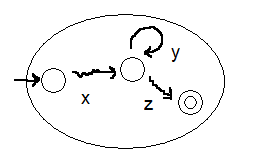
\includegraphics{../18.404/3-6}
\end{center}

Then when $M_1$ reads $xz$ it also goes to the same accept state, so $xz\in L(M_1)$. But $xz$ is shorter than $s=xyz$, contradiction.

Now in order for $M_1$ not to repeat a state, $|s|<k_1$ (if it were longer, a state would repeat by pigeonhole principle. Remember that we have to count the start state too). Similarly, $|s|<k_2$, so $|s|<\max(k_1,k_2)$.
\item
We show the contrapositive: if $U$ includes every string $s$ with $|s|<k_1k_2$, then $U=\Si^*$ (i.e. $U$ includes every string). 

By our proof of closure under union, there exists a DFA with $k_1k_2$ states that recognizes $L(M_1)\cup L(M_2)$ (let the set of states be the product of the set of states of $M_1$ and $M_2$). We claim that if $U$ includes every string $s$ with $|s|<k_1k_2$, then every state of $U$ that is reachable by some string is an accept state.

Let $S(n)$ the set of states reachable after reading in a string of length at most $n$, and let $f(n)=|S(n)|$. Note $f(0)=1$, because we start at the start state.
\begin{clm}
If $f(n)=f(n+1)$, then $S(m)=S(n)$ for all $m\ge n$.
\end{clm}
\begin{proof}
Note $S(n)\subeq S(n+1)$, so $f(n)=f(n+1)$ implies $S(n)=S(n+1)$. This means all arrows coming from states in $S(n)$ go back to states in $S(n+1)$. Thus we can never leave $S(n)$.
\end{proof}
We must have $f(k_1k_2-1)=f(k_1k_2)$, because otherwise $f(0)<f(1)<\cdots <f(k_1k_2)$ and $f(k_1k_2)\ge k_1k_2+1$, contradicting the fact that $M$ has $k_1k_2$ states. Now the fact that $U$ includes every string $s$ with $|s|<k_1k_2$ means that $S(k_1k_2-1)$ consists entirely of accept states. But the lemma gives
\[
S(k_1k_2-1)=S(m),\qquad m>k_1k_2-1,
\]
so $S(k_1k_2-1)$ consists of all the states that are reachable, by a string of any length. Since it consists entirely of accept states, $U=\Si^*$.
\end{enumerate}
\end{problem}

\pagebreak

\begin{problem}{\it(2.19, Tricky grammar)}
$L(G)$ is the language of all strings of $a$'s and $b$'s that is not a number of $a$'s followed by an equal number of $b$'s. Thus
\[
\ol{L(G)}=\set{a^nb^n}{n\ge 0}.
\]
We can represent this by the rules
\begin{align*}
S&\to aSb\\
S&\to \ep.
\end{align*}

\begin{proof}
Let $w\in \{a,b\}^*\bs \set{a^nb^n}{n\ge 0}$. Suppose $w$ has length $n$. Suppose that reading from the front of the string, the first $b$ appears at position $m_1+1$, and reading from the end of the string, the first $a$ appears at position $n-m_2$:
\[
\underbrace{a\ldots a}_{m_1}b\ldots a\underbrace{b\ldots b}_{m_2}.
\]
Note it may be that $m_1$ or $m_2$ is 0. If $b$, $a$ do not appear, then let $m_1=\iy$ and $m_2=\iy$, respectively. Note $w\nin \set{a^nb^n}{n\ge 0}$ ensures that either the $b$ after the $a$'s is not part of the $m_2$ $b$'s, or the $a$ before the $b$'s is not part of the $m_1$ $a$'s.

Now take $m=\min(m_1,m_2)$.
\begin{enumerate}
\item
By applying the rule $S\to aSb$ $m$ times we get
\[
S\stackrel{*}{\implies}\underbrace{a\ldots a}_{m}S\underbrace{b\ldots b}_{m}.
\]
\item
If $m=m_1$ then we apply $S\to bY$ to get 
\[
\underbrace{a\ldots a}_{m=m_1}S\underbrace{b\ldots b}_{m}\implies 
\underbrace{a\ldots a}_{m=m_1}bY\underbrace{b\ldots b}_{m}.
\]
Otherwise we apply $S\to Ya$ to get
\[
\underbrace{a\ldots a}_{m}S\underbrace{b\ldots b}_{m=m_2}\implies 
\underbrace{a\ldots a}_{m}Ya\underbrace{b\ldots b}_{m=m_2}.
\]
\item Now we can use the rules $Y\to bY$ and $Y\to aY$ to fill in the ``middle" the string, from left to right; then terminate by using the rule $Y\to \ep$.
\bal
\underbrace{a\ldots a}_{m=m_1}bY\underbrace{b\ldots b}_{m}&\stackrel{*}{\implies} 
\underbrace{a\ldots a}_{m=m_1}b\cdots \underbrace{b\ldots b}_{m}\\
\text{or }\underbrace{a\ldots a}_{m}Ya\underbrace{b\ldots b}_{m=m_2}&\stackrel{*}{\implies} 
\underbrace{a\ldots a}_{m}\cdots a\underbrace{b\ldots b}_{m=m_2}.
\end{align*}
\end{enumerate}
Note $a^nb^n$ cannot be attained because we are forced to use the rule $S\to aSb$ $n$ times, and then %$\ep$ cannot be attained because at some point
 we must use one of the rules $S\to bY$ or $S\to Ya$, and both these add one more symbol.
\end{proof}
\end{problem}

\pagebreak

\begin{problem}{\it(The class of CFGs is closed under rotational closure)}
\subsection{Motivation}
I try to imitate the proof of Problem 2b, using pushdown automata instead of finite automata. There, the idea is to run the automata starting at state $q$, let it run to an accept state, start it over, and see if the final state is $q$. We take the union over all $q$, using nondeterminism.

Essentially, if the string $x$ takes the machine from $q_0$ to $q$ and $y$ takes the machine from $q$ to $q_a$ (an accept state), then we break up
\begin{equation}\label{eq:404pset-7-a}
q_0\xra{x} q\xra{y}q_a
\end{equation}
into
\begin{equation}\label{eq:404pset-7-b}
q\xra{y} q_a,\qquad q_0\xra{x} q.
\end{equation}
where the first part runs in the first part of the new machine, and the second part runs in the second part of the new machine.
 
But for pushdown automata we have to not only keep track of the {\it state} we're in, but also the {\it state of the stack}.

If we naively imitate the proof with pushdown automata, then we need to take the union over all $q$ and {\it infinitely} many possibilities for the stack. This doesn't work. Instead, we start with an empty stack, but when we have to remove a symbol $a$ from the stack, we have the option of adding instead the new symbol ``$a^{-1}$." These ``inverse" symbols will keep track of what {\it could have been on our stack at state $q$}. (See ``drawing off the stack at $q$" in the proof.) When we get to an accept state, we will have kept track of what we took off our imaginary stack. We have the option of adding more to this imaginary stack, to account for all possibilities for the stack when the machine was in state $q$. (See ``extending the  the stack at $q$" in the proof.) Finally, we run the machine from the start state and see if we end up at an accept state AND end up with this stack. To do this, we have to ``match" the elements that we push onto the stack and their inverses that represent the purported stack at $q$. (See ``checking we get the stack at $q$.")

Here's a good analogy: originally the stack at $q$ is covered in dirt, so we don't see anything---we think it's empty. An inverse symbol $a^{-1}$ means ``aha, I think I've unearthed $a$ from the buried stack." There might be more symbols that we haven't unearthed, so we may have to guess at them (``extend" the stack).
\subsection{Proof}
Suppose $A$ is a CFG. We can find a pushdown automaton $M=(Q,\Si,\Ga,\de,q_0,F)$ that recognizes $A$. For each state $q$ of $M$ define the pushdown automaton $M_q$ as follows:
\begin{itemize}
\item The stack alphabet of $M_q$ is the disjoint union of two copies of $\Ga$ and an extra symbol ``\$." If $a$ is in $\Ga$, then let the other copy of $a$ be ``$a^{-1}$."
\item
$M_q$ is made of 2 copies of $M$, say $M_1$ and $M_2$, with some modifications as described below.
\item
Let the starting state of $M_q$ be a new state $s$. Add a $\ep,\ep\to \$$ transition from $s$ to the start state of $M_1$. Here, $\$$ is a symbol that represents ``This is the bottom of the stack."
\item (``Drawing off the stack at $q$")
For each transition in $M_1$
\tikzstyle{state}=[circle,draw,inner sep=1pt,minimum size=6mm]
\tikzstyle{accept}=[circle,draw,inner sep=4pt,minimum size=7.5mm]
\begin{center}
\begin{tikzpicture}[->,>=stealth',shorten >=1pt,auto,node distance=1cm,semithick]
\node (q1) [state] {$q_1$};
\node (q2) at (2,0) [state] {$q_2$};
\path (q1) edge node {$a,\,b\to c$} (q2);
\end{tikzpicture}
\end{center}
we add the following to the diagram:
\begin{equation}\label{eq:404pset-7-1}
\begin{tikzpicture}[->,>=stealth',shorten >=1pt,auto,node distance=1cm,semithick]
\node (q1) [state] {$q_1$};
\node (q2) at (2,0) [state] {$q_2$};
\node (qt) at (1,-1) [state] {$q_t$};
\path (q1) edge [swap] node {$a,\,\ep\to b^{-1}$} (qt);
\path (qt) edge [swap] node {$\ep,\,\ep\to c$} (q2);
\end{tikzpicture}
\end{equation}
where $q_t$ is a new, unique node assigned to the transition. Basically, the $b^{-1}$ represents the fact we're taking off a $b$ that we ``guessed" to exist in the stack at $q$.
\item (``Extending the stack at $q$")
Add two more states $r_1,r_2$. Add an $\ep,\ep\to \ep$-transition from each accept state of $M_1$ to $r_1$, and from $r_2$ to the start state of $M_2$. For every symbol $a\in \Si$, add a $\ep, a\to \ep$ transition from $r_1$ to $r_1$ (``removing the final stack"), add $\ep,\,a^{-1}\to a^{-1}$ and $\ep,\$\to \$$ from $r_1$ to $r_2$ (``forcing removal of the final stack"),  and $\ep, \ep\to a^{-1}$ transition from $r_2$ to $r_2$ (``extending the stack at $q$"). (This is more transparent when you read claims 2 and 3 on the next page.)
\begin{center}
\begin{tikzpicture}[->,>=stealth',shorten >=1pt,auto,node distance=1cm,semithick]
\node (s) {$M_1$};
\node (r1) at (0,-1.5) [state] {$r_1$};
\node (r2) at (0,-3) [state] {$r_2$};
\node (s2) at (0,-4.5) {$M_2$};
\path (r1) edge [loop right] node {$\ep, a\to \ep\;\forall a$} (r1);
\path (r2) edge [loop right] node {$\ep, \ep\to a^{-1}\;\forall a$} (r2);
\path (s) edge node {$\ep,\,\ep\to \ep$} (r1);
\path (r1) edge node{$\ep,\,\$\to \$,\,a^{-1}\to a^{-1}\forall a$} (r2);
\path (r2) edge node{$\ep,\,\ep\to \ep$} (s2);
\end{tikzpicture}
\end{center}

%Note the inverses were added on in reverse order, so adding more inverses at $r_2$ corresponds to ``guessing" what could have been at the bottom of the stack at $q$, which we haven't touched. 
\item (``Checking we get the stack at $q$")
For each transition in $M_2$
\begin{center}
\begin{tikzpicture}[->,>=stealth',shorten >=1pt,auto,node distance=1cm,semithick]
\node (q1) [state] {$q_1$};
\node (q2) at (2,0) [state] {$q_2$};
\path (q1) edge node {$a,\,b\to c$} (q2);
\end{tikzpicture}
\end{center}
we add the following to the diagram:
\begin{equation}\label{eq:404pset-7-2}
\begin{tikzpicture}[->,>=stealth',shorten >=1pt,auto,node distance=1cm,semithick]
\node (q1) [state] {$q_1$};
\node (q2) at (2,0) [state] {$q_2$};
\node (qt) at (1,-1) [state] {$q_t$};
\path (q1) edge [swap] node {$a,\,b\to \ep$} (qt);
\path (qt) edge [swap] node {$\ep,\,c^{-1}\to \ep$} (q2);
\end{tikzpicture}
\end{equation}
where $q_t$ is a new, unique node assigned to the transition.

Basically, instead of adding $c$, we have the option of ``matching" it up with a $c^{-1}$ already on the stack. Recall that the $c^{-1}$ represents an element we guessed would be on the stack when we got to $q$.
\item (When to accept)
Declassify all accept states. Add an accept state $q_a$, and an $\ep,\,\$\to \ep$-transition from $q$ to $q_a$.
\begin{center}
\begin{tikzpicture}[->,>=stealth',shorten >=1pt,auto,node distance=1cm,semithick]
\node (s) [state] {$q$};
\node (r1) at (0,-1.5) [state] {$q_a$};
\node (r2) at (0,-1.5) [accept] {$q_a$};
\path (s) edge node {$\ep,\,\$\to \ep$} (r1);
\end{tikzpicture}
\end{center}
\end{itemize}
\begin{clm}
$M_q$ recognizes exactly those strings of the form $yx$ where $xy\in A$ and some thread of $M$ is in state $q$ after reading $x$.
\end{clm}\label{clm:787-1-7}
Given this claim, it remains to note that
\[
RC(M)=\bigcup_q L(M_q)
\]
because for $xy\in A$, $M$ is in {\it some} state $q$ after reading $x$. The union of CFG's is a CFG (the proof is the same as the proof for regular languages), so $RC(M)$ is a CFG.
\begin{proof}[Proof of claim]
%Indeed, to get to the accept state in $M_q$, we have to follow the $\ep$ transition from $M_1$ to $M_2$ sometime.
%
%Let $y$ be the string read before that transition and $x$ be the string read after that transition. In $M_1$, we went from $q$ to an accept state $q_a$ after reading $y$, and in $M_2$ we went from the start state $q_s$ to $q$ after reading $x$.
%\begin{gather*}
%q\xra{y} q_a\\
%q_s\xra{x} q.
%\end{gather*}
%
%Then in the original machine $M$, the machine goes from the start state to $q$ after reading $x$ and from $q$ to an accept state after reading $y$:
%\[
%q_s\xra{x}q\xra{y}q_a.
%\]
%Conversely, given $x,y$ like this, $yx$ would be recognized by $M_q$.
We claim that if the machine $M_q$ accepts a string $w$, then the following must be true {\it of the thread that led to the accept state}. Let $y$ be the part of the string read in the first part $M_1$ and $x$ the the part of the string read in the second part $M_2$.
\begin{enumerate}
\item
At every time in $M_1$, there can be no inverse symbol (such as $a^{-1}$) above a symbol in the original stack language (such as $a$). Thus right after exiting $M_1$, the stack, read top to bottom, looks like $a_1\ldots a_mb_n^{-1}\cdots b_1^{-1}$.
\item
Suppose right after exiting $M_1$, the stack, read top to bottom, is $a_1\ldots a_mb_n^{-1}\cdots b_1^{-1}$. Then we could have started at state $q$ in $M$, with a stack $b_1\ldots b_n$, and finished at an accept state of $M$ after reading $x$, with a stack $a_1\ldots, a_m$. (Conversely, such a series of steps in $M$ corresponds to such a series of steps in $M_q$.)
\item
We could also have started at state $q$ in $M$ with a stack $b_1\ldots b_{n+k}$, for any $b_{n+1},\ldots, b_{n+k}$ and traversed the exact same steps to finish at the same accept state of $M$. 
\item
When $M_q$ enters the second part $M_2$, there can be no symbol in the original language $\Ga$ on the stack. Hence, the stack must look like $b_{n+k}^{-1}\cdots b_1^{-1}$.
\item
If the stack is $b_{n+k}^{-1}\cdots b_1^{-1}$ when it enters $M_2$, then in the original machine $M$ we could have arrived at $q$ with a stack $b_1\cdots b_{n+k}$ after reading $m$. 
\end{enumerate}
Sketches of the proofs are as follows.
\begin{enumerate}
\item
If there is an inverse symbol above a symbol $a$ at any time in $M_1$, then it will persist when we leave $M_1$. We can never remove $a$---we can't remove it at $r_1$, and nothing allows us to remove it in $M_2$. Thus, we can't reach the bottom of the stack, marked by $\$$, to accept.

Intuitively, putting an inverse symbol above a symbol in the original language means we're claiming to remove stuff we didn't know was on the stack, when we already have stuff we know to be on the stack, which doesn't make sense. 
\item
This is by construction of~\eqref{eq:404pset-7-1}. Adding $b^{-1}$ and then $c$ to the stack in $M_q$ corresponds to popping $b$ from the stack and pushing $c$ in $M$.
\item
Clear.
\item
There is no way to get rid of this symbol.
\item
This is by construction of~\eqref{eq:404pset-7-2}. Pushing $c$ onto the stack in $M$ can correspond to popping $c^{-1}$ off the stack in $M_q$.
\end{enumerate}
%We have two more claims that tell us {\it step by step} what is going on in $M_1$ and $M_2$.
%
%With all these claims, one can prove without too much difficulty that if $M$ reads $x$ and arrives at state $q$ with stack $a
%
%When $M_2$ is reading $x$, it proceeds the same way as if $M$ were reading $x$, except that it may follow
Claim~\ref{clm:787-1-7} is clear from combining the claims. The picture is as in~\eqref{eq:404pset-7-a} and~\eqref{eq:404pset-7-b} with the extra data of what is on the stack at state $q$.
\end{proof}
\end{problem}

\end{document}

